\section{Inheritance}
 
\emph{
	``The inheritance permit to a class to be 
	used in a modified form when a sub-class 
	is derived from it''
} \cite{Capretz:2003}. This O-O resource 
can be used as a way to define new
classes based in more general classes 
that have been 
defined previously, acquiring their characteristics.  
If a class \emph{CurrentTransformer} directly 
inherits from class \emph{Transformer} we say that 
\emph{Transformer} is the parent 
of \emph{CurrentTransformer} and 
\emph{CurrentTransformer} is the 
child of \emph{Transformer} \cite{Snyder:1986}. 
The UML representation is given in 
Figure \ref{fig:inheritance-fig}.

\begin{figure}
  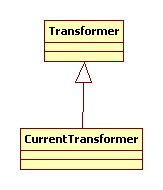
\includegraphics[width=0.3\textwidth]{chapters/ch-oop/figures/inheritance}
  \caption{
  		Inheritance: \emph{Transformer} is the parent 
		of \emph{CurrentTransformer}
%Observation: Long sentences don't work with list of figures.		 
%		and 
%		\emph{CurrentTransformer} is the 
%		child of \emph{Transformer}
		}
  \label{fig:inheritance-fig}
\end{figure}

The inheritance is a great resource to create 
reusable code and common informations and methods 
thanks to hierarchical classes. 
Various techniques to write reusable code are 
avaliable 
\cite{Johnson:1988} 
\cite{Micallef:1988}
\cite{Gossain:1990} 
\cite{Capretz:1992}.  
\todo[inline]{mejorar la abreb. de estas 2 
	primeras bibliografias. Los nombres 
	completos pueden encontrarse en
	http://portal.acm.org/citation.cfm?id=638778&dl=ACM&coll=portal&CFID=4389858&CFTOKEN=67060785#
}
